\section{Quadcopter flight tests}

\todo[inline]{Resumen del flight plan}

\subsection{Build process}
\label{sec:test-7-builddrone}

% Setup:    build drone, configuration, calibration
% Test:     - RC, GPS, 
%           - Arm, takeoff commands
%           - Camera holder
% Results:  wiring, drone pictures, QGroundControl calibration screens
%           holder 3d, drone close-up, camera feed

Once the performance and safety of the control algorithms has been validated in the simulated environment, it is possible to begin flight tests and take to the air with a physical drone.
As has been mentioned before, the vehicle used in this project is the Holybro X500, designed specifically to work with PX4.
The detailed instructions to build the vehicle from its Development Kit can be found in the PX4 documentation\footnote{\url{https://docs.px4.io/main/en/frames_multicopter/holybro_x500_pixhawk4.html}}.
Figure \ref{fig:x500-dev-kit} shows all the parts that make up the complete vehicle.
\todo[inline]{Show own image of complete build here}

\begin{figure}
  \centering
  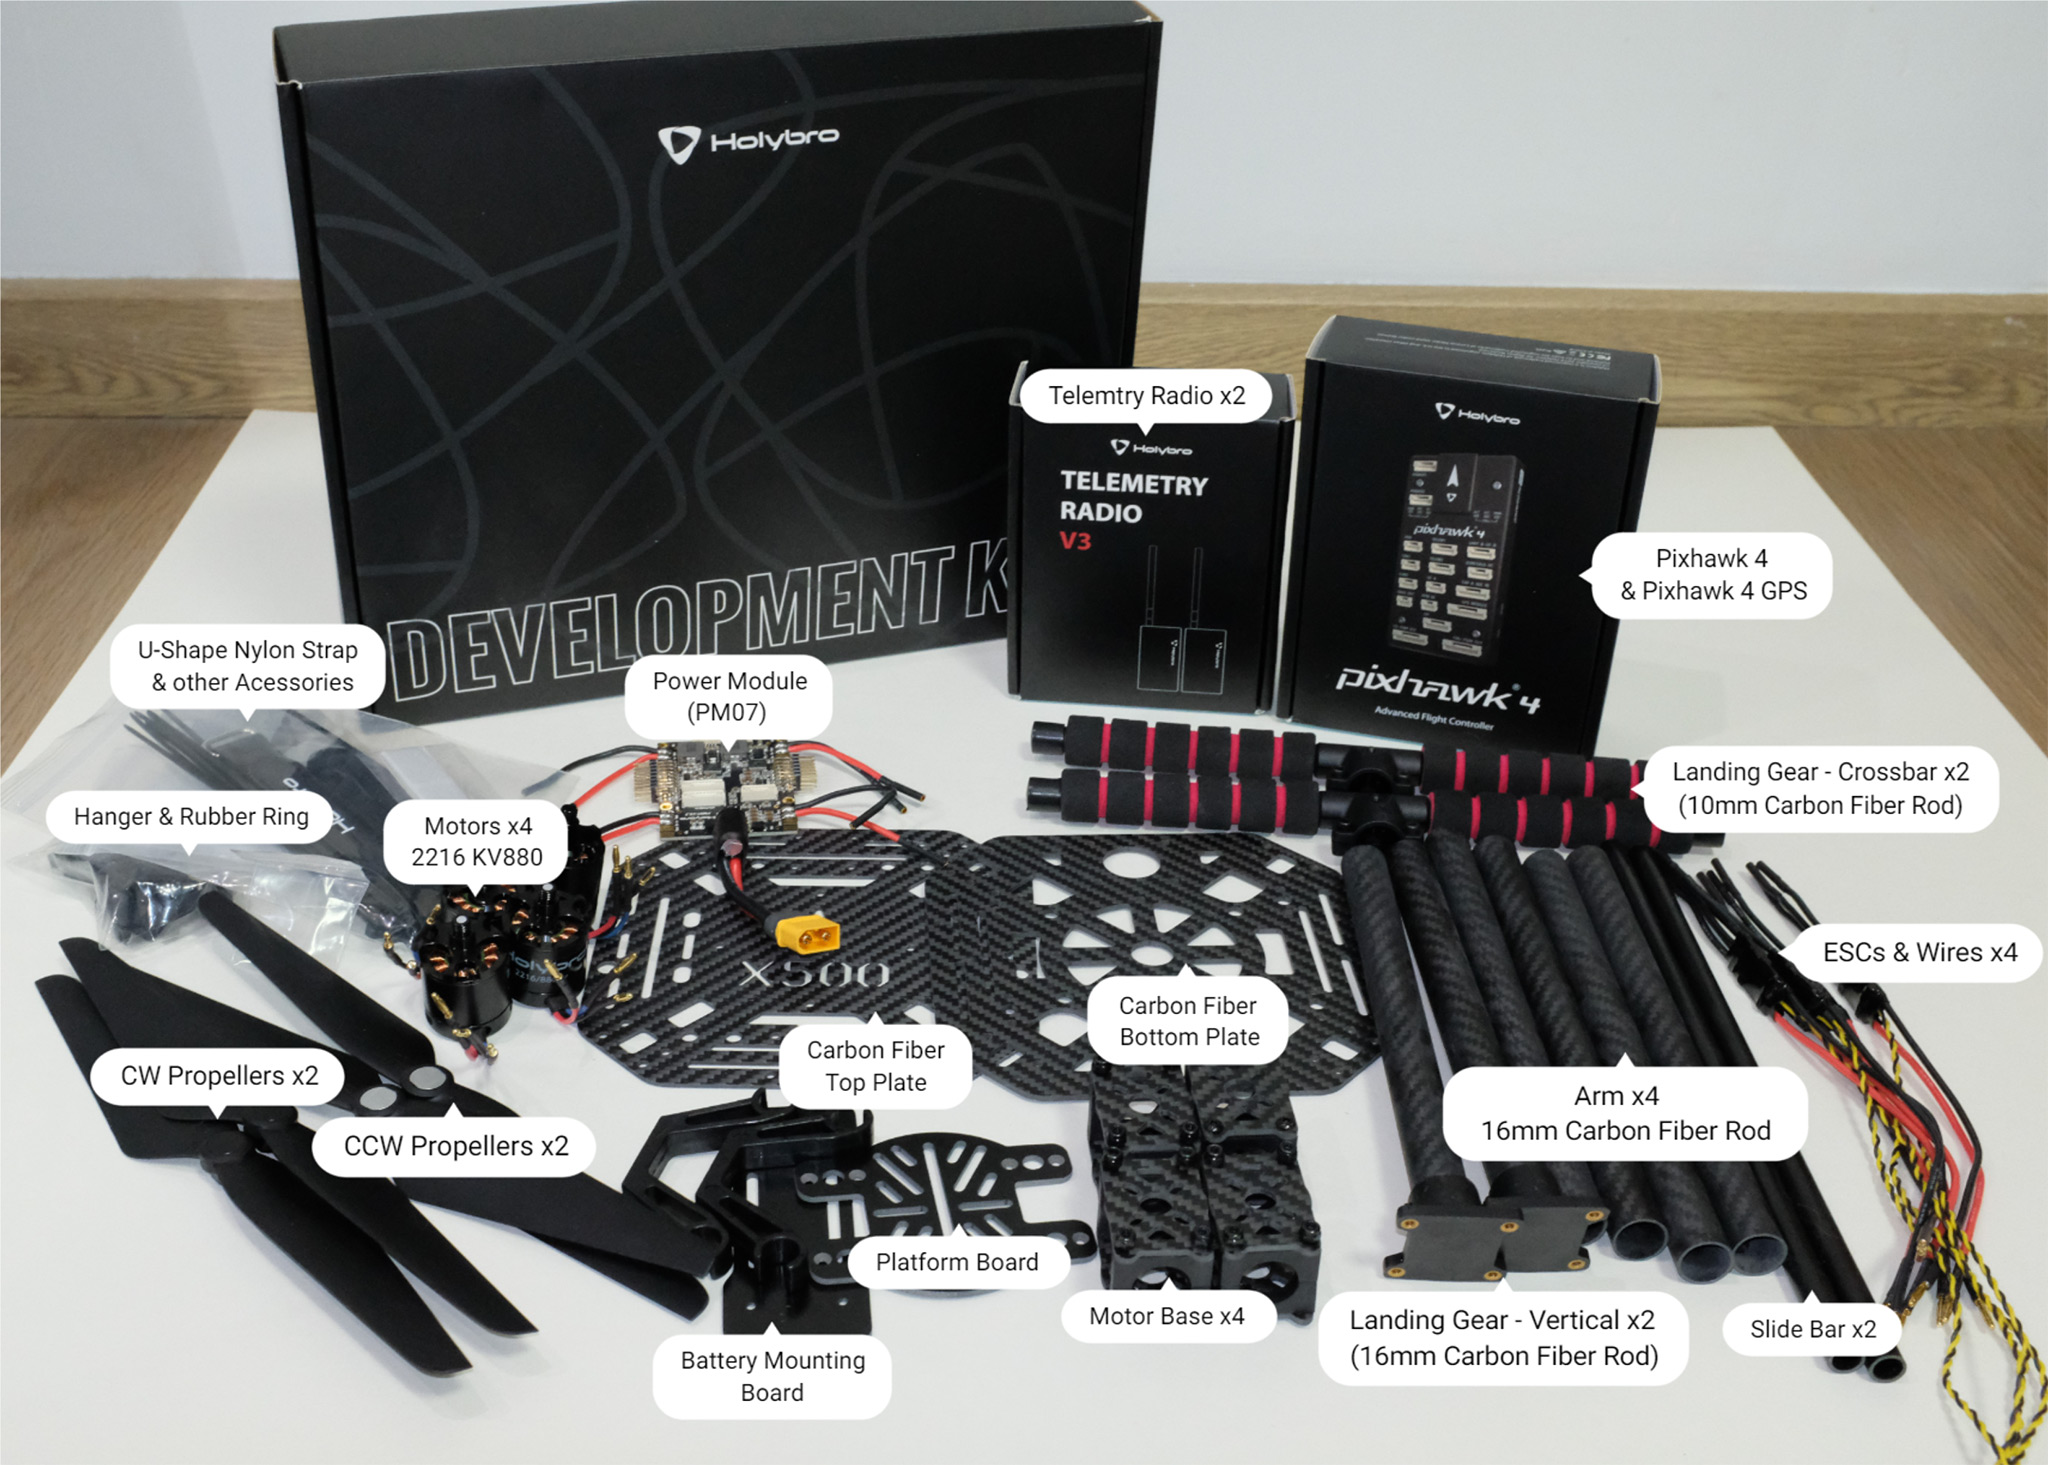
\includegraphics[width=.6\textwidth, keepaspectratio]{img/x500-dev-kit.jpg}
  \caption{Development kit for the Holybro X500}\label{fig:x500-dev-kit}
  \todo{Cite}
\end{figure}

After the vehicle has been built, there are additional installation and calibration steps that must be carried out before it can fly.
The QGroundControl \ref{subsec:qgc} ground station application contains a configuration screen with all the calibration tools needed for the vehicle setup, as shown in figure \ref{fig:qgc-config}.

\begin{figure}
  \centering
  
\includegraphics[width=\textwidth, keepaspectratio]{img/placeholder.png}
  \caption{Screenshot from the QGroundControl calibration and setup tools used to configure the vehicle}\label{fig:qgc-config}
\end{figure}

The vehicle can be configured either by connecting the flight controller directly to the computer via the micro-USB port on its side or through a wireless connection by plugging the companion telemetry radio to the computer running QGroundControl.
Once the vehicle is fully configured, the RC controller or QGroundControl can be used to test assisted take off and landing.
At this point, the drone should be able to maintain stable flight while using autopilot-assisted flight modes like Position Mode, where the roll and pitch sticks control the acceleration over ground of the vehicle in the forward/backward and left/right directions relative to the heading the vehicle is facing, and throttle controls speed of ascent and descent. 
With the sticks centered the vehicle will actively remain locked to a position in 3D space, compensating for wind and other forces.
This is the safest manual mode to test that all the default components are working as expected before adding the companion computer and the onboard camera.

\todo[inline]{Power supply starts here, there's mention on the hitl part that should be here}

While in flight the Raspberry Pi will be powered through \todo{power supply} so and so.

The camera needs to be attached to the frame of the vehicle in a secure way.
For this purpose, a support has been designed and 3D-printed from PLA plastic.
The holder attaches to the slide bars underneath the main frame of the vehicle so that the camera and its substantial weight is situated as close to the center of mass as possible, between the battery and the GPS platform.
The 3D model of the custom support can be seen in figure \ref{fig:camera-holder-3d}.
Figure \ref{fig:camera-holder-overall} shows how the underside of the vehicle looks with the camera attached.

\subsection{Basic tests}
\label{sec:test-8-flight}

% Setup:    flight plan
% Test:     - assisted takeoff, fly with RC
%           - tools/test_camera + record video
% Results:  video of flying, adjust pid set-point

In this section, all the final composing parts will be tested together as the final step before running the developed control solutions in real flight.
With the help of the camera testing tool the following points need to be checked:
\begin{enumerate}
    \item The companion computer can run the necessary application while powered via battery
    \item The companion computer can establish a serial connection with the flight controller in normal run mode (HITL disabled)
    \item The dronecontrol application can send takeoff and landing commands that are carried out by the vehicle
    \item The camera can record images with a perspective and frame rate appropriate for human detection and following
\end{enumerate}

\begin{figure}
  \centering
  
\includegraphics[width=.6\textwidth, keepaspectratio]{img/placeholder.png}
  \caption{Picture from flight tests}\label{fig:flight-test-basic}
\end{figure}

\begin{figure}
  \centering
  
\includegraphics[width=.6\textwidth, keepaspectratio]{img/placeholder.png}
  \caption{Pose detection algorithm running on images taken during flight}\label{fig:flight-test-cam}
\end{figure}


\subsection{Hand gesture control}
\label{sec:test-9-hand}

% Setup:    ...
% Test:     - Hand solution on windows through telemetry radio
%           - Free movement with offboard api
% Results:  video of flying, output from program

\subsection{Target detecting, tracking and following}
\label{sec:test-10-follow}

% Setup:    ...
% Test:     - Follow solution on RPi
%           - Controller response to real input
% Results:  video of flying, output from program
